

\begin{frame}{Desmatamento e Queimadas}
  Monitoramento automatizado de áreas onde o desmatamento ilegal ultrapassa 10.000 km²/ano, permitindo ações de comando e controle em tempo real.
  \begin{figure}
    \centering
    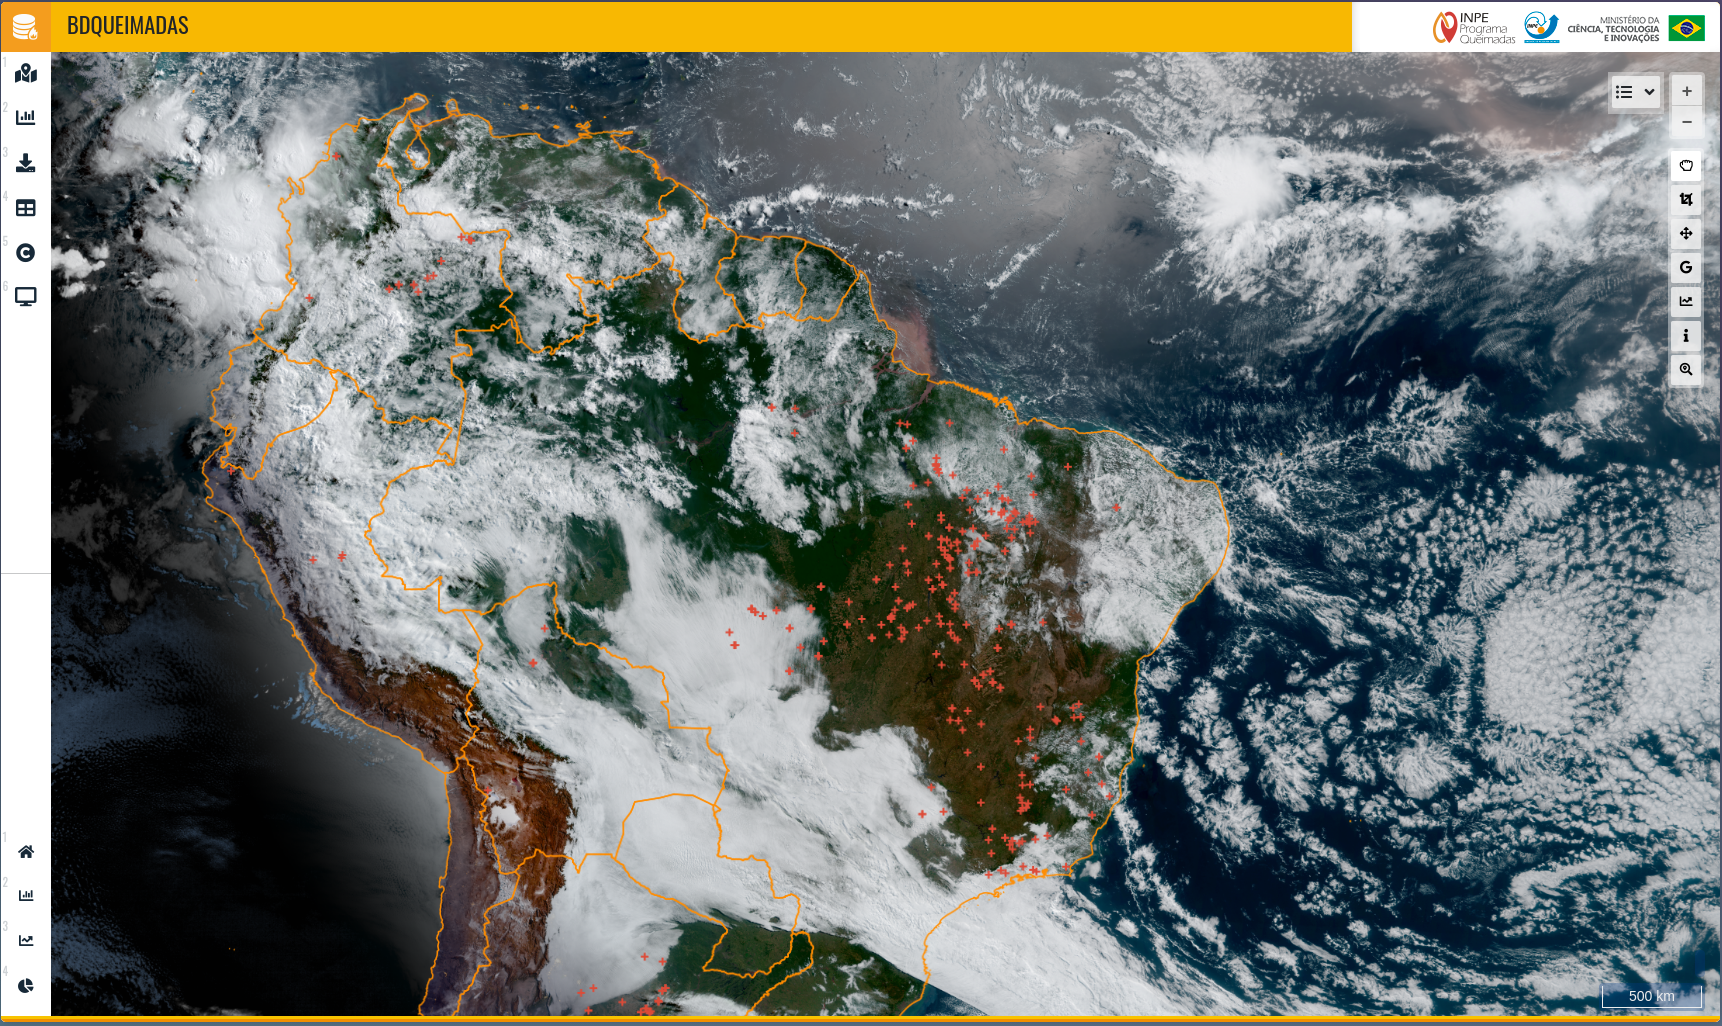
\includegraphics[width=0.6\textwidth]{introducao/INPE_queimadas.png}
    \\
    \footnotesize Foto do programa BDQueimadas do INPE (Instituto Nacional de Pesquisas Espaciais)
  \end{figure}
\end{frame}

\begin{frame}{Desmatamento e Queimadas}
  \vspace{0.5em}
  \begin{columns}
    \column{0.48\textwidth}
      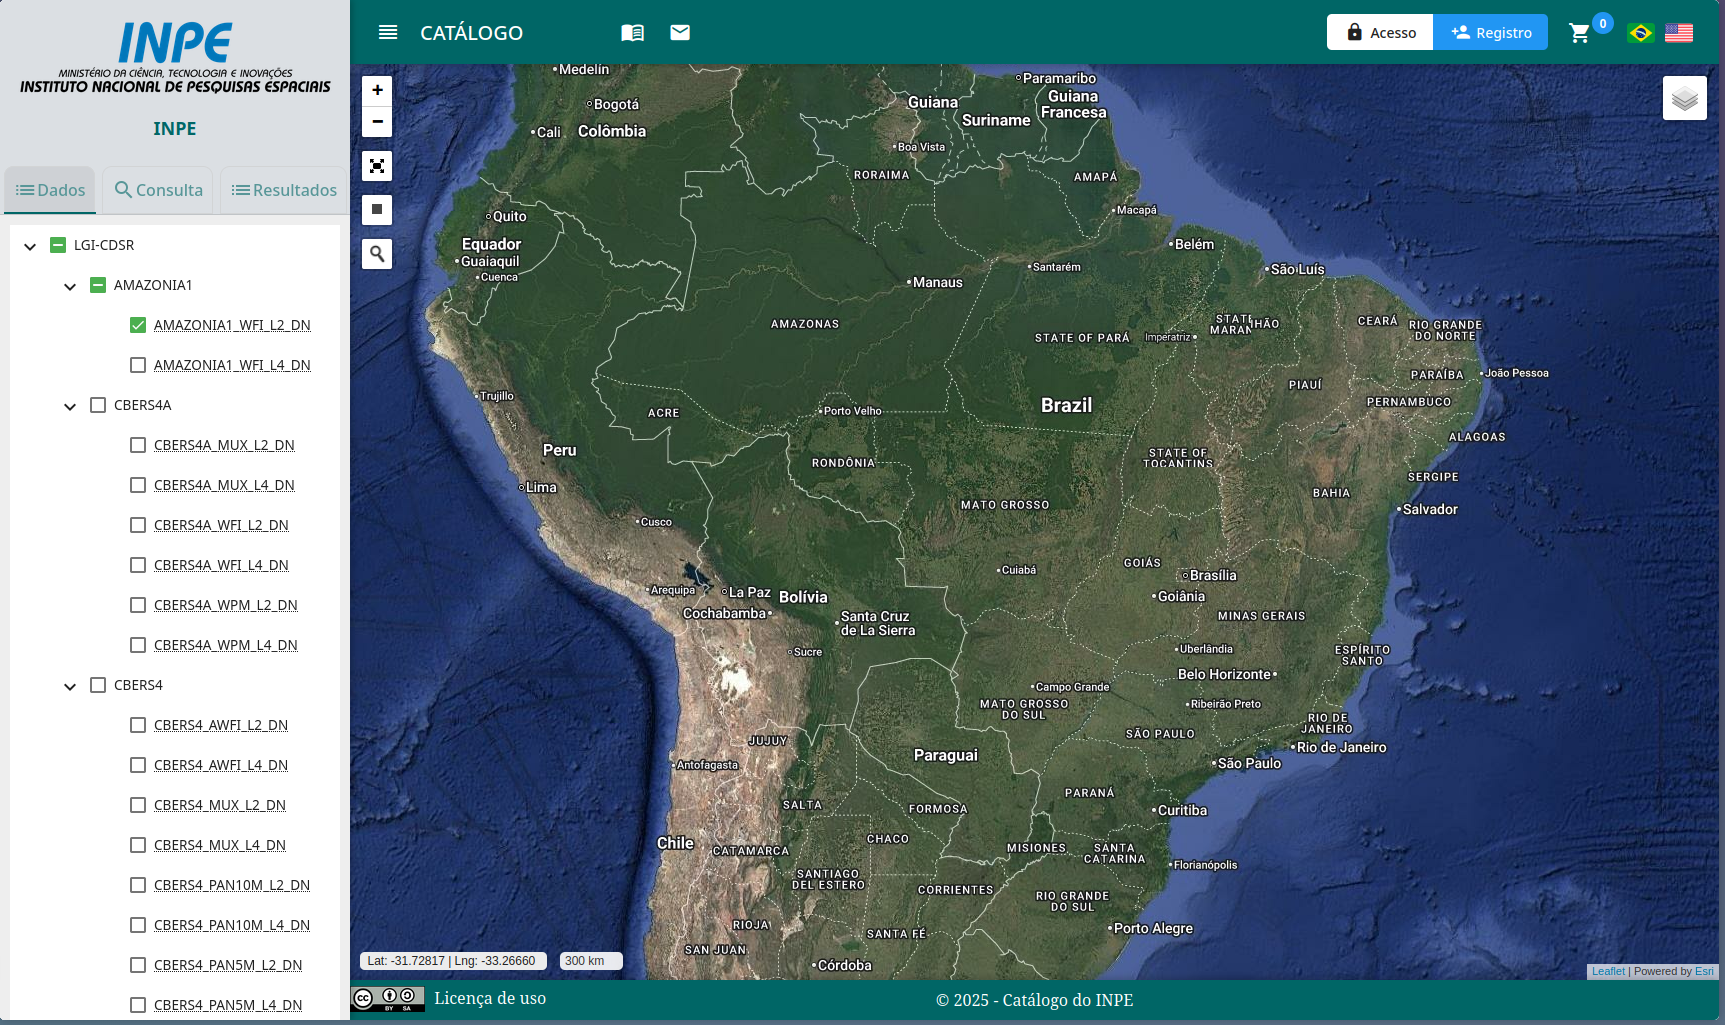
\includegraphics[width=\textwidth]{introducao/INPE_satelite1.png}
    \column{0.48\textwidth}
      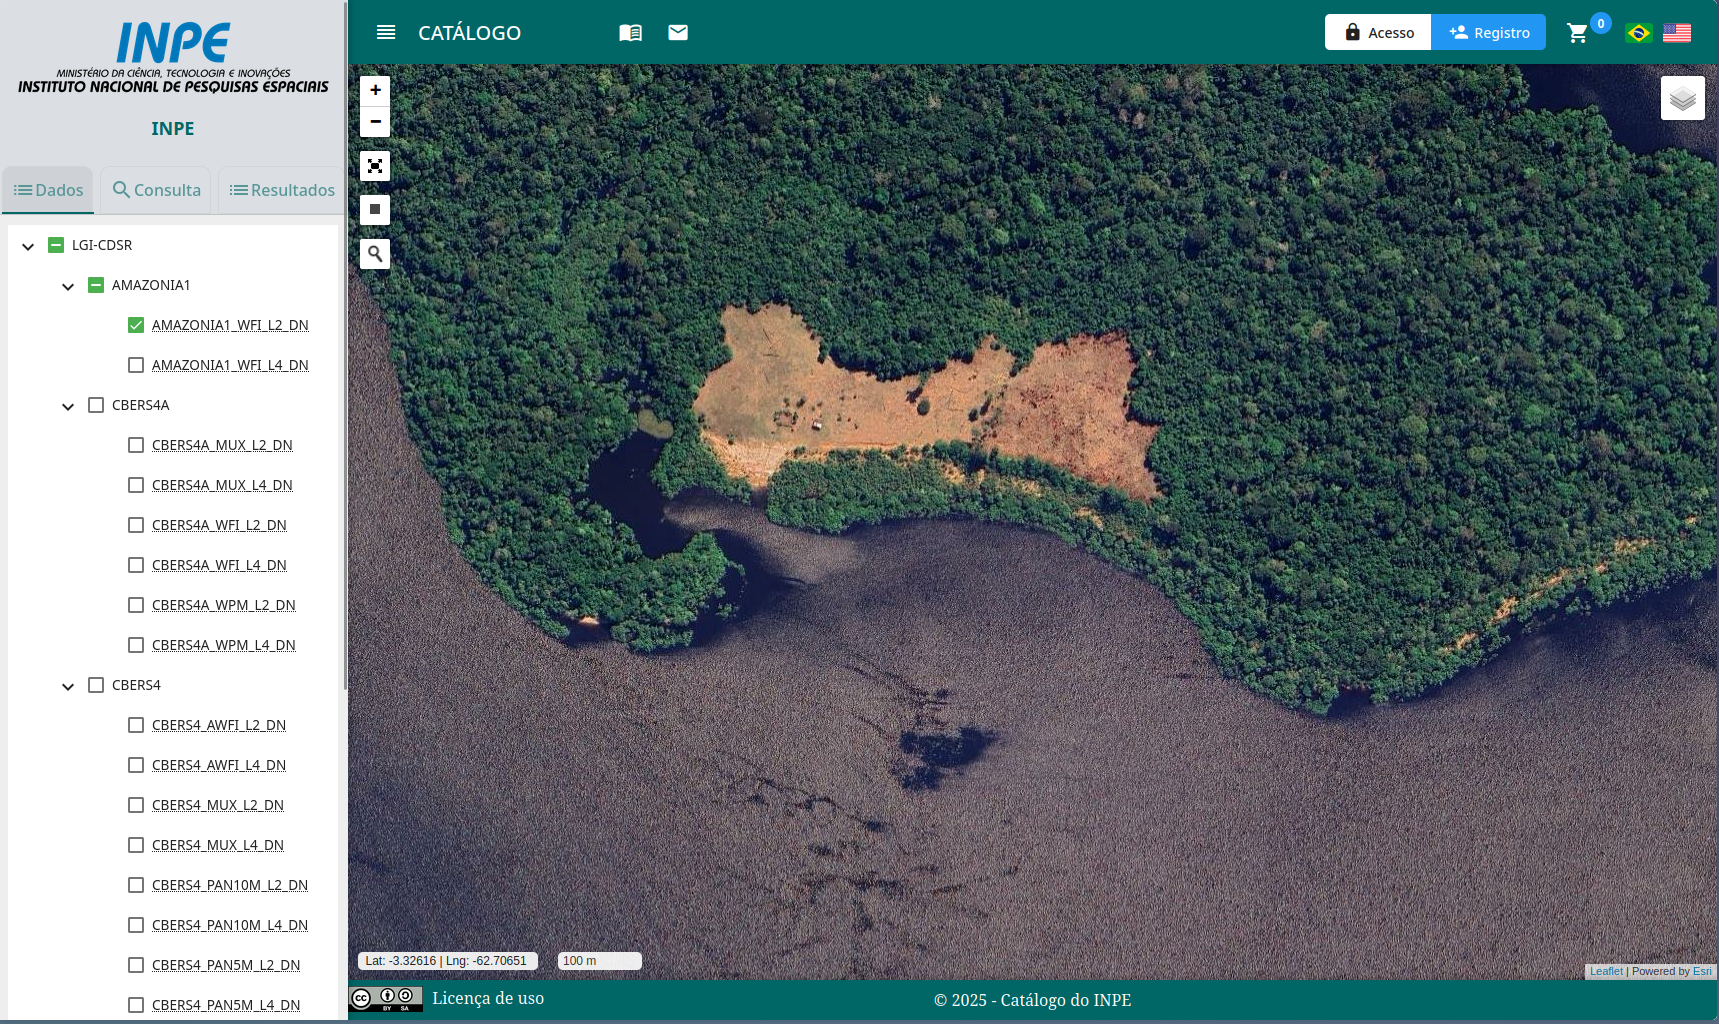
\includegraphics[width=\textwidth]{introducao/INPE_satelite2.png}
  \end{columns}
  \vspace{0.5em}
  \centering
  \footnotesize Fotos de satélite disponíveis no catálogo do INPE
\end{frame}

\begin{frame}{Infraestrutura clandestina}
  Detecção de pistas de pouso improvisadas na TI Yanomami que abastecem o garimpo ilegal e ameaçam comunidades indígenas.
 \begin{figure}
    \centering
    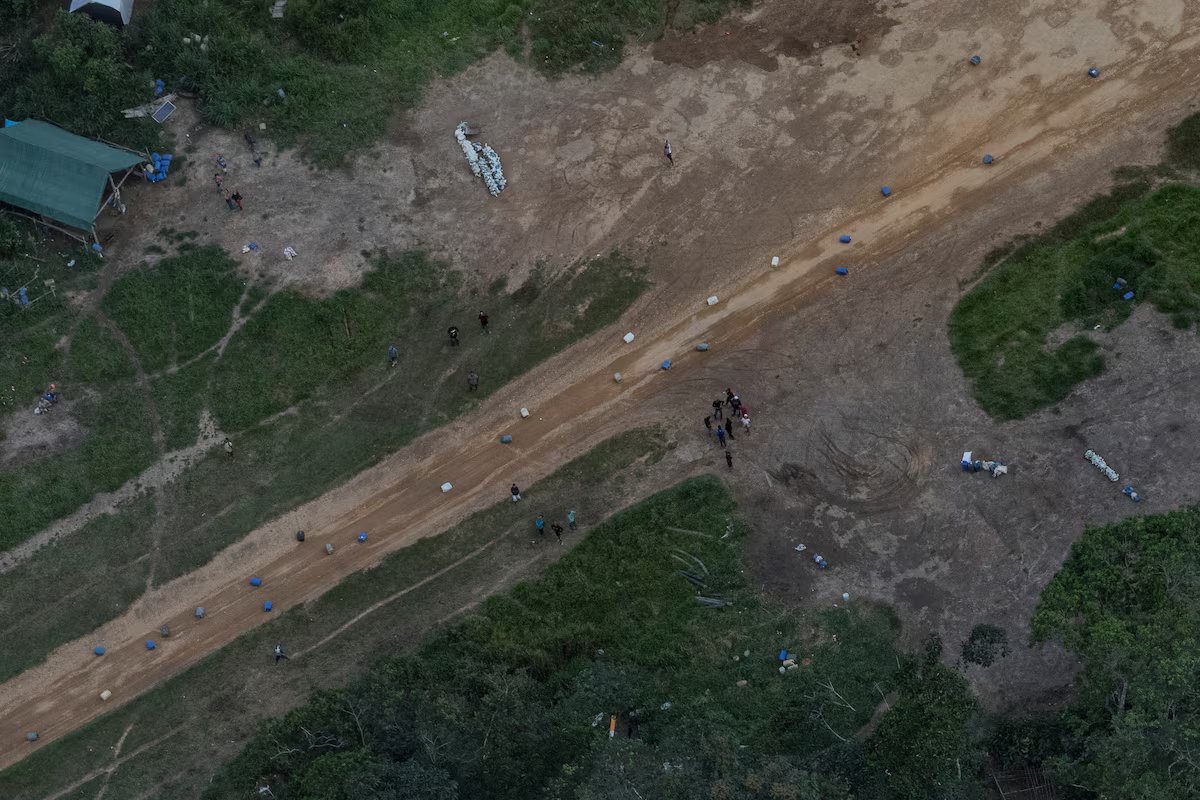
\includegraphics[width=0.4\textwidth]{introducao/foto_satelite_pista.png}
    \\
    \footnotesize Garimpeiros espalham tambores de combustível ao longo de pistas ilegais na Amazônia para impedir pousos. Foto: Victor Moriyama/The New York Times
  \end{figure}
  
\end{frame}

\begin{frame}{Desastres climáticos}
  Mapeamento de enchentes como as de 2024 no Rio Grande do Sul (90\% do estado inundado, com mais de 581.000 pessoas afetadas), otimizando rotas de evacuação e envio de recursos de emergência.
\end{frame}

\begin{frame}{Inteligência geopolítica}
  Classificação de áreas críticas em cenários de conflito (ex.: recente escalada Israel × Irã) para suporte a decisões estratégicas de defesa.

  \begin{figure}
    \centering
    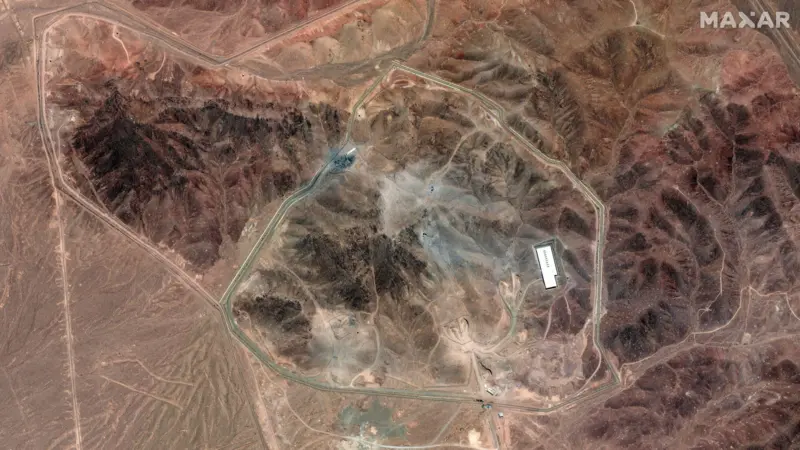
\includegraphics[width=0.6\textwidth]{introducao/satelite_ira.png}
    \\
    \footnotesize Imagem de satélite da instalação de enriquecimento de combustível de Fordo, no Irã, após os ataques aéreos de 23 de junho.
  \end{figure}
  
\end{frame}
